% TEMPLATE for Usenix papers, specifically to meet requirements of
%  USENIX '05
% originally a template for producing IEEE-format articles using LaTeX.
%   written by Matthew Ward, CS Department, Worcester Polytechnic Institute.
% adapted by David Beazley for his excellent SWIG paper in Proceedings,
%   Tcl 96
% turned into a smartass generic template by De Clarke, with thanks to
%   both the above pioneers
% use at your own risk.  Complaints to /dev/null.
% make it two column with no page numbering, default is 10 point

% Munged by Fred Douglis <douglis@research.att.com> 10/97 to separate
% the .sty file from the LaTeX source template, so that people can
% more easily include the .sty file into an existing document.  Also
% changed to more closely follow the style guidelines as represented
% by the Word sample file. 

% Note that since 2010, USENIX does not require endnotes. If you want
% foot of page notes, don't include the endnotes package in the 
% usepackage command, below.

% This version uses the latex2e styles, not the very ancient 2.09 stuff.

% NOTE: use end-notes, not footnotes
%Citation example:
%Now we're going to cite somebody.  Watch for the cite tag.
%Here it comes~\cite{Chaum1981,Diffie1976}.  The tilde character (\~{})
%in the source means a non-breaking space.  This way, your reference will
%always be attached to the word that preceded it, instead of going to the
%next line.

\documentclass[letterpaper,twocolumn,10pt]{article}
\usepackage{usenix,epsfig,graphicx,float,url,longtable,enumitem,array}
\setlist{nolistsep}

\newcolumntype{L}[1]{>{\raggedright\let\newline\\\arraybackslash\hspace{0pt}}p{#1}}

\newcommand{\comment}[1]{}
\begin{document}

%don't want date printed
\date{}

%make title bold and 14 pt font (Latex default is non-bold, 16 pt)
\title{\Large \bf Give Your Data the Edge: A Scalable Data Delivery Platform}

\author{\rm Larry Peterson (PI)\\
llp@cs.princeton.edu\\
\emph{NSF 1541318}
}

\maketitle

% Use the following at camera-ready time to suppress page numbers.
% Comment it out when you first submit the paper for review.
\thispagestyle{empty}

\setlength{\parskip}{0pt}
\setlength{\parsep}{0pt}
\setlength{\headsep}{0pt}
\setlength{\topskip}{0pt}
\setlength{\topmargin}{0pt}
\setlength{\topsep}{0pt}
\setlength{\partopsep}{0pt}

Science is increasingly data-driven.  Collaborators regularly tap data from
multiple repositories across the world to generate even more data for others to
consume.  Effective science requires effective data management, but most scientists are
not experts in distributed storage.  To address this, we created Syndicate, a
general-purpose scalable storage system that automates data retrieval, staging,
and storage across multiple sites.

Syndicate offers a sustainable way for curating scientific data with an emphasis
on ease-of-use.  It interfaces with legacy data storage systems,
commodity cloud storage, and content distribution networks (CDNs) to create coherent
read/write storage volumes that span multiple sites and attach to scientists' VMs and laptops like
removable drives.  Using only her workstation, a PI can select datasets and
storage infrastructure, create volumes, and add collaborator user accounts, and the system
will automatically configure itself at runtime.

The most significant challenge in the design and implementation of Syndicate
is to provide end-to-end data gurarantees like consistency, durability, and
availability.  End-to-end consistency is particularly
tricky because data analysis tools assume very particular consistency
models, but the underlying infrastructure offers variable and often very weak
guarantees.  For example, BLAST interacts with data under POSIX
consistency semantics, but an Amazon S3 bucket augmented with a CDN can at best
provide delta consistency.

Mismatches like this result in lots of ``glue code'' to make
scientific software interoperate with storage infrastructure.  Glue code is
workflow- and storage-specific, and maintaining it requires deep knowledge of
both.  This imposes high operational costs, since
any changes mean throwing out and
writing more glue code to preserve compatibility.

\begin{figure}[ht!]
   \centering
   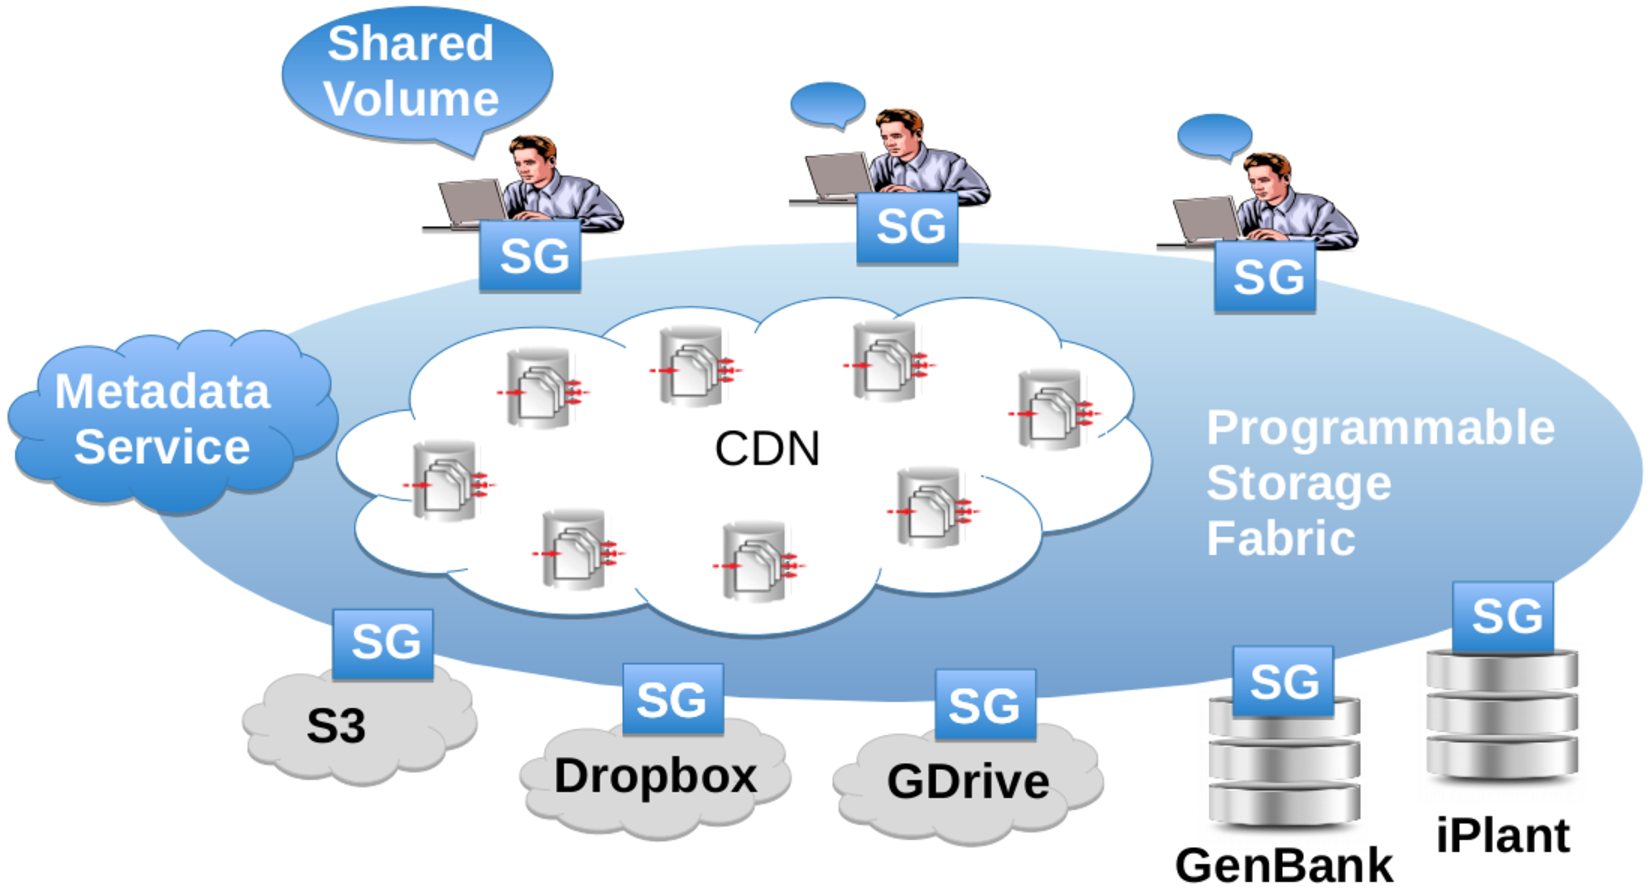
\includegraphics[width=0.5\textwidth]{fig2.pdf}
   \caption{\it Syndicate deployment.  Drivers run in gateways (SG), which
   coordinate via a Metadata Service.  Together, they make up the programmable
   storage fabric that links existing infrastructure together to create shared
   volumes.}
   \label{fig:syndicate-overview}
\end{figure}

Syndicate overcomes this challenge with a novel storage programming model that
replaces bespoke glue code with \emph{composable, reusable storage drivers}
running in a \emph{programmable storage fabric} that spans the wide-area
(Figure~\ref{fig:syndicate-overview}).
Once written, a Syndicate driver can be deployed and combined with other drivers
and used in other workflows to provide the desired end-to-end consistency.

To achieve this, Syndicate provides built-in snapshot isolation on files ``on top'' of 
the storage infrastructure.  Data chunks are \emph{immutable}
between writes, and have \emph{globally-unique addresses} in the system.
Whole-chunk \texttt{get}s, \texttt{put}s, and \texttt{delete}s never conflict,
which lets users implement consistency simply by constraining the order in which
chunks are processed relative to other chunks.  By separating data storage and
retrieval from operation ordering, we enable consistency-preserving logic to be developed
independently of both the workflow and storage provider.

We have deployed Syndicate on OpenCloud to give each user a shared volume
for accessing data across compute clusters.  Users attach iRODS deployments
to an Akamai CDN and commodity storage to accelerate data delivery across the
wide-area and automatically stage it to compute clusters.  The CDN's weak
consistency does \emph{not} affect workflow correctness.  We have achieved this
with only a few hundred lines of Python in the drivers.

\end{document}

